\begin{figure*}[t!]
\centering
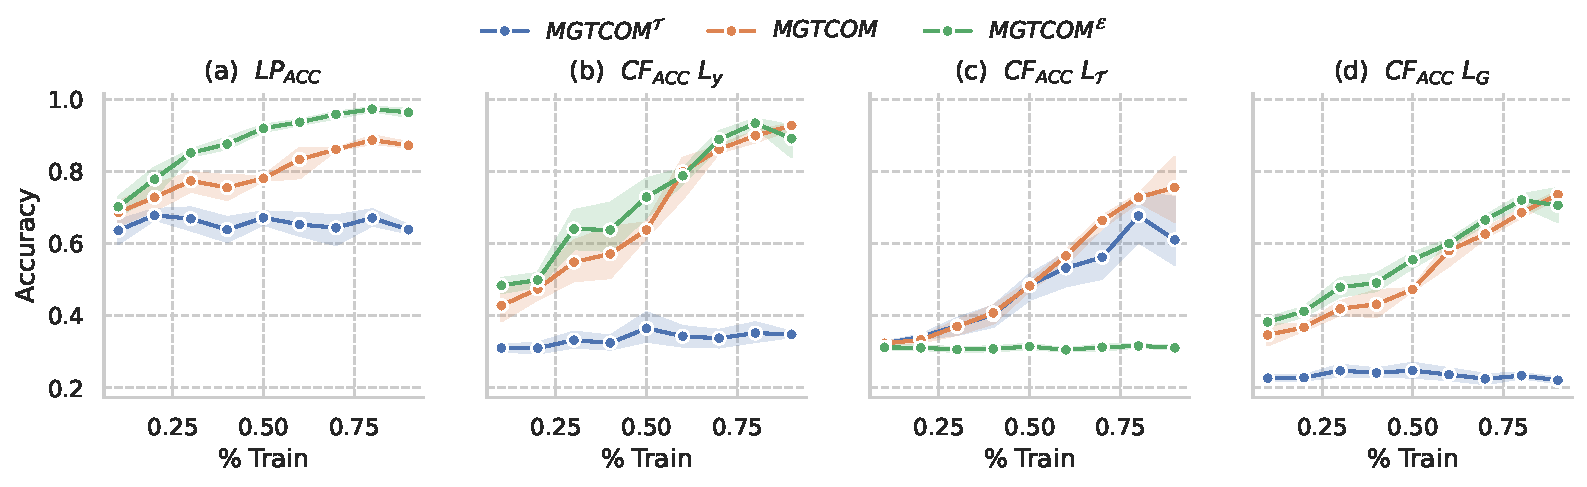
\includegraphics[width=\textwidth]{resources/figs/inference.pdf}
\caption{
    Visual comparison of different model variants in the inference-based setting. 
    Graph nodes are split into three disjointed sets (train, validation, and test).
    The metrics are measured while the training to validation ratio is varied. 
    The test set is set to 10\% of the nodes and is kept constant.
    The average metrics per data value are plotted along with their standard deviation.
}
\label{fig:inference}
\end{figure*}    